\documentclass[portrait,a0,final,20pt]{a0poster}
%%%Load packages
\usepackage{multicol} 			%2-column layout
% \setlength\columnsep{8pt} % This is the default columnsep for all pages
\usepackage[left=2cm,right=2cm,bottom=2cm,top=0cm]{geometry}			%Reset margins
\usepackage{helvet}				%Load Helvetica font & CM math
\usepackage{color}				%Needed for colour boxes & coloured text
% \usepackage{graphics}
\usepackage{graphicx}
\usepackage{subcaption}
\usepackage[font=Large,labelfont=bf]{caption}
\usepackage{float}
\usepackage{tikz}
\usetikzlibrary{arrows,positioning, shapes.symbols,shapes.callouts,patterns,shapes,chains,calc,backgrounds,fadings}

\usepackage[absolute,overlay]{textpos} % for logo next ti title

\usepackage{titlesec}
\usepackage{tabularx, booktabs} % make width of table columns evenly distributed (see http://tex.stackexchange.com/questions/60601/evenly-distributing-column-widths)

\usepackage{enumitem}
\usepackage{animate}[2017/05/18]

\usepackage[hidelinks, colorlinks = true,
            linkcolor = blue,
            urlcolor  = blue,
            citecolor = blue,
            anchorcolor = blue]{hyperref}
\usepackage{xcolor}
\usepackage{newtxtext,newtxmath}

\usepackage[noend]{algorithm2e}
\newcommand\mycommfont[1]{\footnotesize\ttfamily\textcolor{blue}{#1}}
\SetCommentSty{mycommfont}

\usepackage{amssymb} 
\usepackage{pifont}% for red cross and green tick

% \usepackage{titlepic}
% \usepackage{columns}

\titlespacing\section{0pt}{10pt plus 4pt minus 2pt}{5pt plus 2pt minus 2pt}
\titlespacing\subsection{0pt}{12pt plus 4pt minus 2pt}{0pt plus 2pt minus 2pt}

\titleformat*{\section}{\Huge\bfseries}
\titleformat*{\subsection}{\Large\bfseries}
\titleformat*{\subsubsection}{\large\bfseries}
\titleformat*{\paragraph}{\large\bfseries}
\titleformat*{\subparagraph}{\large\bfseries}

%%%Define colours and lengths
\definecolor{headingcol}{rgb}{0,0,0}			%Colour of main title
\definecolor{boxcol}{rgb}{0.7,0.2,0.2}		%Edge-colour of box and top banner
\fboxsep=1cm							%Padding between box and text
\setlength{\columnsep}{2cm}				%Set spacing between columns
\renewcommand{\familydefault}{\sfdefault}	%Set main text to sans-serif

%%%Format title
\makeatletter							%Needed to include code in main file
\renewcommand\@maketitle{%
\null									%Sets position marker
% \vspace{5em}
{
\color{headingcol}\sffamily\VeryHuge \textbf		%Set title font and colour
\@title \par}%
% \vskip 0.6em%
{
\color{black}\sffamily\LARGE				%Set author font and colour
\lineskip .5em%
\begin{tabular}[t]{l}%
\@author
\end{tabular}\par}%
\vskip 1cm
\par
}
\makeatother



\title{Disease Knowledge Transfer across Neurodegenerative Diseases}

\newcommand{\inst}[1]{$^{#1}$}

% \author{\Large{R\u{a}zvan V. Marinescu\inst{1}, Neil P. Oxtoby\inst{1}, Alexandra L. Young\inst{1}, Arman Eshaghi\inst{2}, Peter A. Wijeratne\inst{1}, Daniel C. Alexander\inst{1}}\\
% \begin{tabular}{l p{1cm} l p{1cm} l}
% \large{$^1$Centre for Medical Image Computing, University College London}  & & \large{$^2$Queen Square MS Centre, UCL Institute of Neurology} \\
% \end{tabular}
% }

% \author{\LARGE{R\u{a}zvan Marinescu\inst{1,2}, Marco Lorenzi\inst{3}, Stefano Blumberg\inst{1}, Alexandra Young\inst{1}, Pere Morell\inst{1}},\\ \LARGE{Neil Oxtoby\inst{1}, Arman Eshaghi\inst{1,4}, Keir Yong\inst{5}, Sebastian Crutch\inst{5}, Polina Golland\inst{2}, Daniel Alexander\inst{1}}\\}

\author{\LARGE{R\u{a}zvan V. Marinescu, Marco Lorenzi, Stefano B. Blumberg, Alexandra L. Young, Pere Morell},\\ \LARGE{Neil Oxtoby, Arman Eshaghi, Keir Yong, Sebastian Crutch, Polina Golland, Daniel C. Alexander}\\}

% \begin{tabular}{l p{1cm} l p{1cm} l}
% \large{$^1$Centre for Medical Image Computing, UCL, UK}  & & \large{$^3$University of C\^{o}te d'Azur, Inria Sophia Antipolis, France} & & \large{$^5$Dementia Research Centre, UCL, UK}\\
% \large{$^2$Computer Science and Artificial Intelligence Laboratory, MIT, USA} & & \large{$^4$Queen Square MS Centre, UCL Institute of Neurology, UK} & & 
%  \\
% \end{tabular}
 

% \institute{Centre for Medical Image Computing, University College London, UK
% \and 
% Computer Science and Artificial Intelligence Laboratory, MIT, USA
% \email{razvan@csail.mit.edu}
% \and
% Queen Square MS Centre, UCL Institute of Neurology, UK
% \and 
% Dementia Research Centre, University College London, UK
% \and
% University of C\^{o}te d'Azur, Inria Sophia Antipolis, France
% % Laboratoire d'Analyse Num\'{e}rique, B\^{a}timent 425,\\
% % F-91405 Orsay Cedex, France}
% }

\newcommand{\fnt}[1]{\LARGE{#1}}

\DeclareMathOperator*{\argmin}{arg\,min}
\DeclareMathOperator*{\argmax}{arg\,max}


\begin{document}
							%Align with edge of page, not margin
% \vspace{2cm}
% \includegraphics[scale=1,trim=0 0 0 200, clip]{Black_Landscape.pdf}
\hspace{-1cm}	
\begin{minipage}{50cm}					%Minipage for title contents
% \vspace{-18cm}
\maketitle
\end{minipage}
\begin{textblock}{0}(9.95,0.2)
\begin{tabular}{l}

\includegraphics[height=5.5cm]{mit_logo}
\includegraphics[height=5.5cm]{inria_logo}
\includegraphics[height=6cm]{qr_dkt.png}\\
\hspace{11.45cm}
\includegraphics[height=5cm]{ucl_logo}\\
\end{tabular}


\end{textblock}

\fnt{


\newcommand{\lp}{\lambda_{d_i}^{k}}
\newcommand{\lpuu}{\lambda_{d_i}^{k,(u)}}
\newcommand{\lpum}{\lambda_{d_i}^{k,(u-1)}}

\newcommand{\cmark}{\ding{51}}%
\newcommand{\xmark}{\ding{55}}%

\newcommand{\yes}{{\LARGE \textcolor{green!50!black}{\cmark} \par}}
\newcommand{\no}{{\LARGE \textcolor{red}{\xmark} \par}}

\vspace{0.2em}
\hrule
\vspace{0.2em}

\newcommand{\heading}[1]{\noindent\textbf{\Huge{#1}}}

\begin{multicols}{2}							
\raggedcolumns							%Don't stretch contents vertically

\pagenumbering{gobble}

%%%Column1
\vspace{-3em}

\heading{Aim:}\;\;\;\;Infer progression of multimodal biomarkers in rare neurodegenerative diseases (NDs) by leveraging larger datasets of common NDs.


\heading{Why:}\;\;\;\;Posterior Cortical Atrophy (PCA): progression of \underline{multimodal} biomarkers not known $\rightarrow$ Identify outcome measures and suitable subjects for PCA clinical trials.

\columnbreak

% \heading{Challenges}
% 
% \begin{figure}[H]
% \fnt{
% 
% \begin{subfigure}{0.48\columnwidth}
%  
%    Rare Neurodeg. Diseases
%   
%   \begin{itemize}
%    \item Small datasets \no
%    \item MRI only \no
%    \item Cross-sectional \no
% %    \item Poorly understood \no
%   \end{itemize}
%  
% \end{subfigure}
%  }
% \end{figure}

\begin{figure}[H]
 \centering
 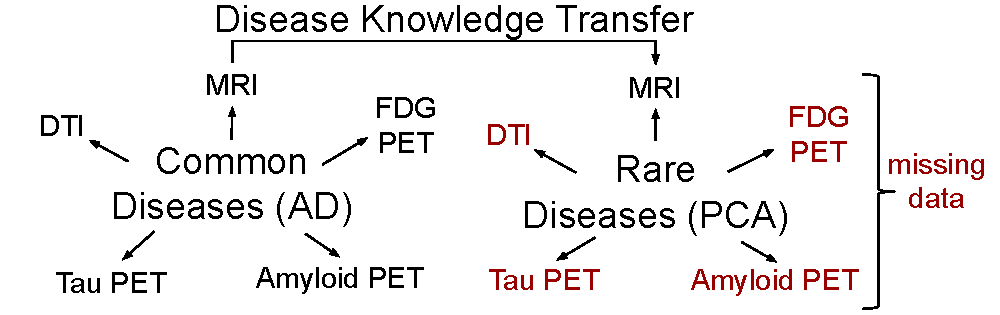
\includegraphics[width=\columnwidth]{DKT_data_availability}
\end{figure}


\end{multicols}
\hrule
\vspace{0.2em}

\begin{multicols}{2}							
\raggedcolumns	

\heading{1. Intuition}

\begin{itemize}
 \item Diseases affect different brain regions un-equally, but underlyining mechanisms are the same (amyloid cascade).
 \item \textbf{Idea:} each brain region follows ``its own disease course'', common across diseases.
\end{itemize}

\begin{figure}[H]

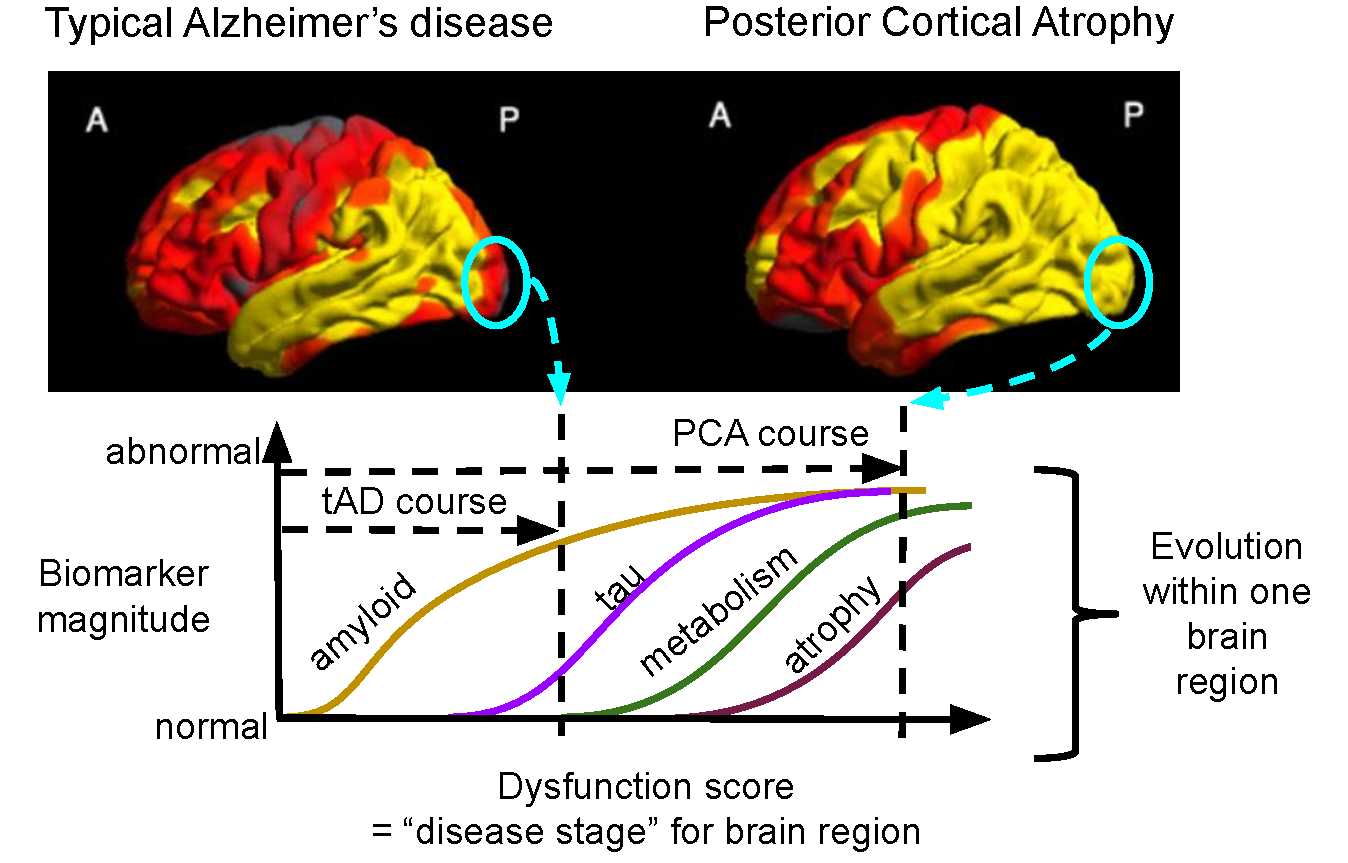
\includegraphics[width=\columnwidth]{DKT_intuition}
 
\end{figure}


\heading{2. Method}
 
\vspace{0.6em}
\begin{figure}[H]
 \centering
   \begin{subfigure}{0.49\columnwidth}
   \centering
   \fnt{1. Each disease characterised by region-specific dysfunction trajectories}\\
   $ \gamma_{ij}^l = f(\beta_{i} + m_{ij}; \lambda_{d_i}^l) $\\
%    \vspace{0.9em}
%    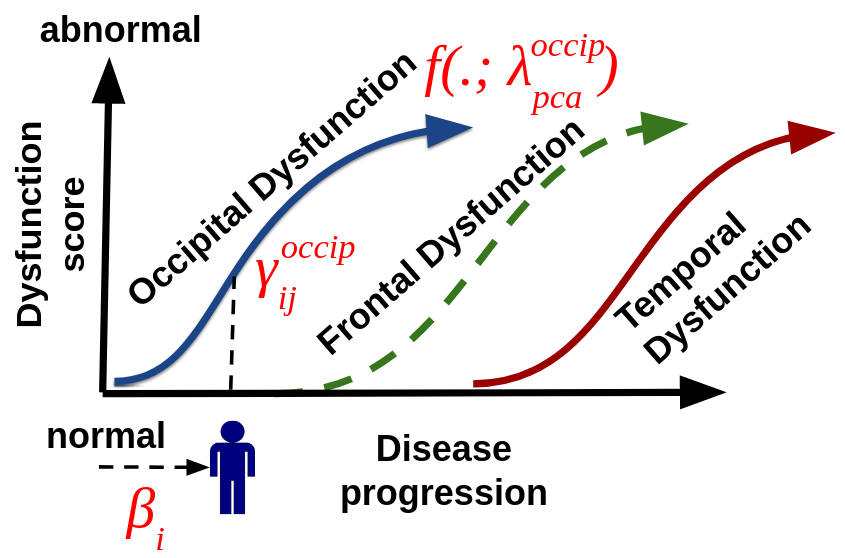
\includegraphics[width=\textwidth]{diseaseEvol}
   
  \end{subfigure}
  \begin{subfigure}{0.49\columnwidth}
   \centering
%    \vspace{-1.2em}
   \fnt{2. Dysfunction trajectory modelled using region-specific biomarkers}\\
   $ y_{ijk} = g( \gamma_{ij}^{k} ; \theta_k) + N(0,\epsilon_k) $
%    \vspace{0.6em}
%    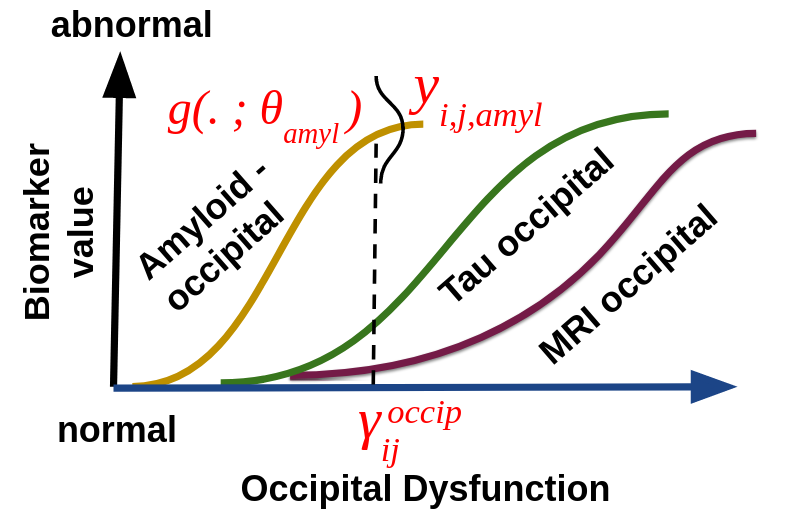
\includegraphics[width=\textwidth]{dysfuncEvol}
  \end{subfigure}

 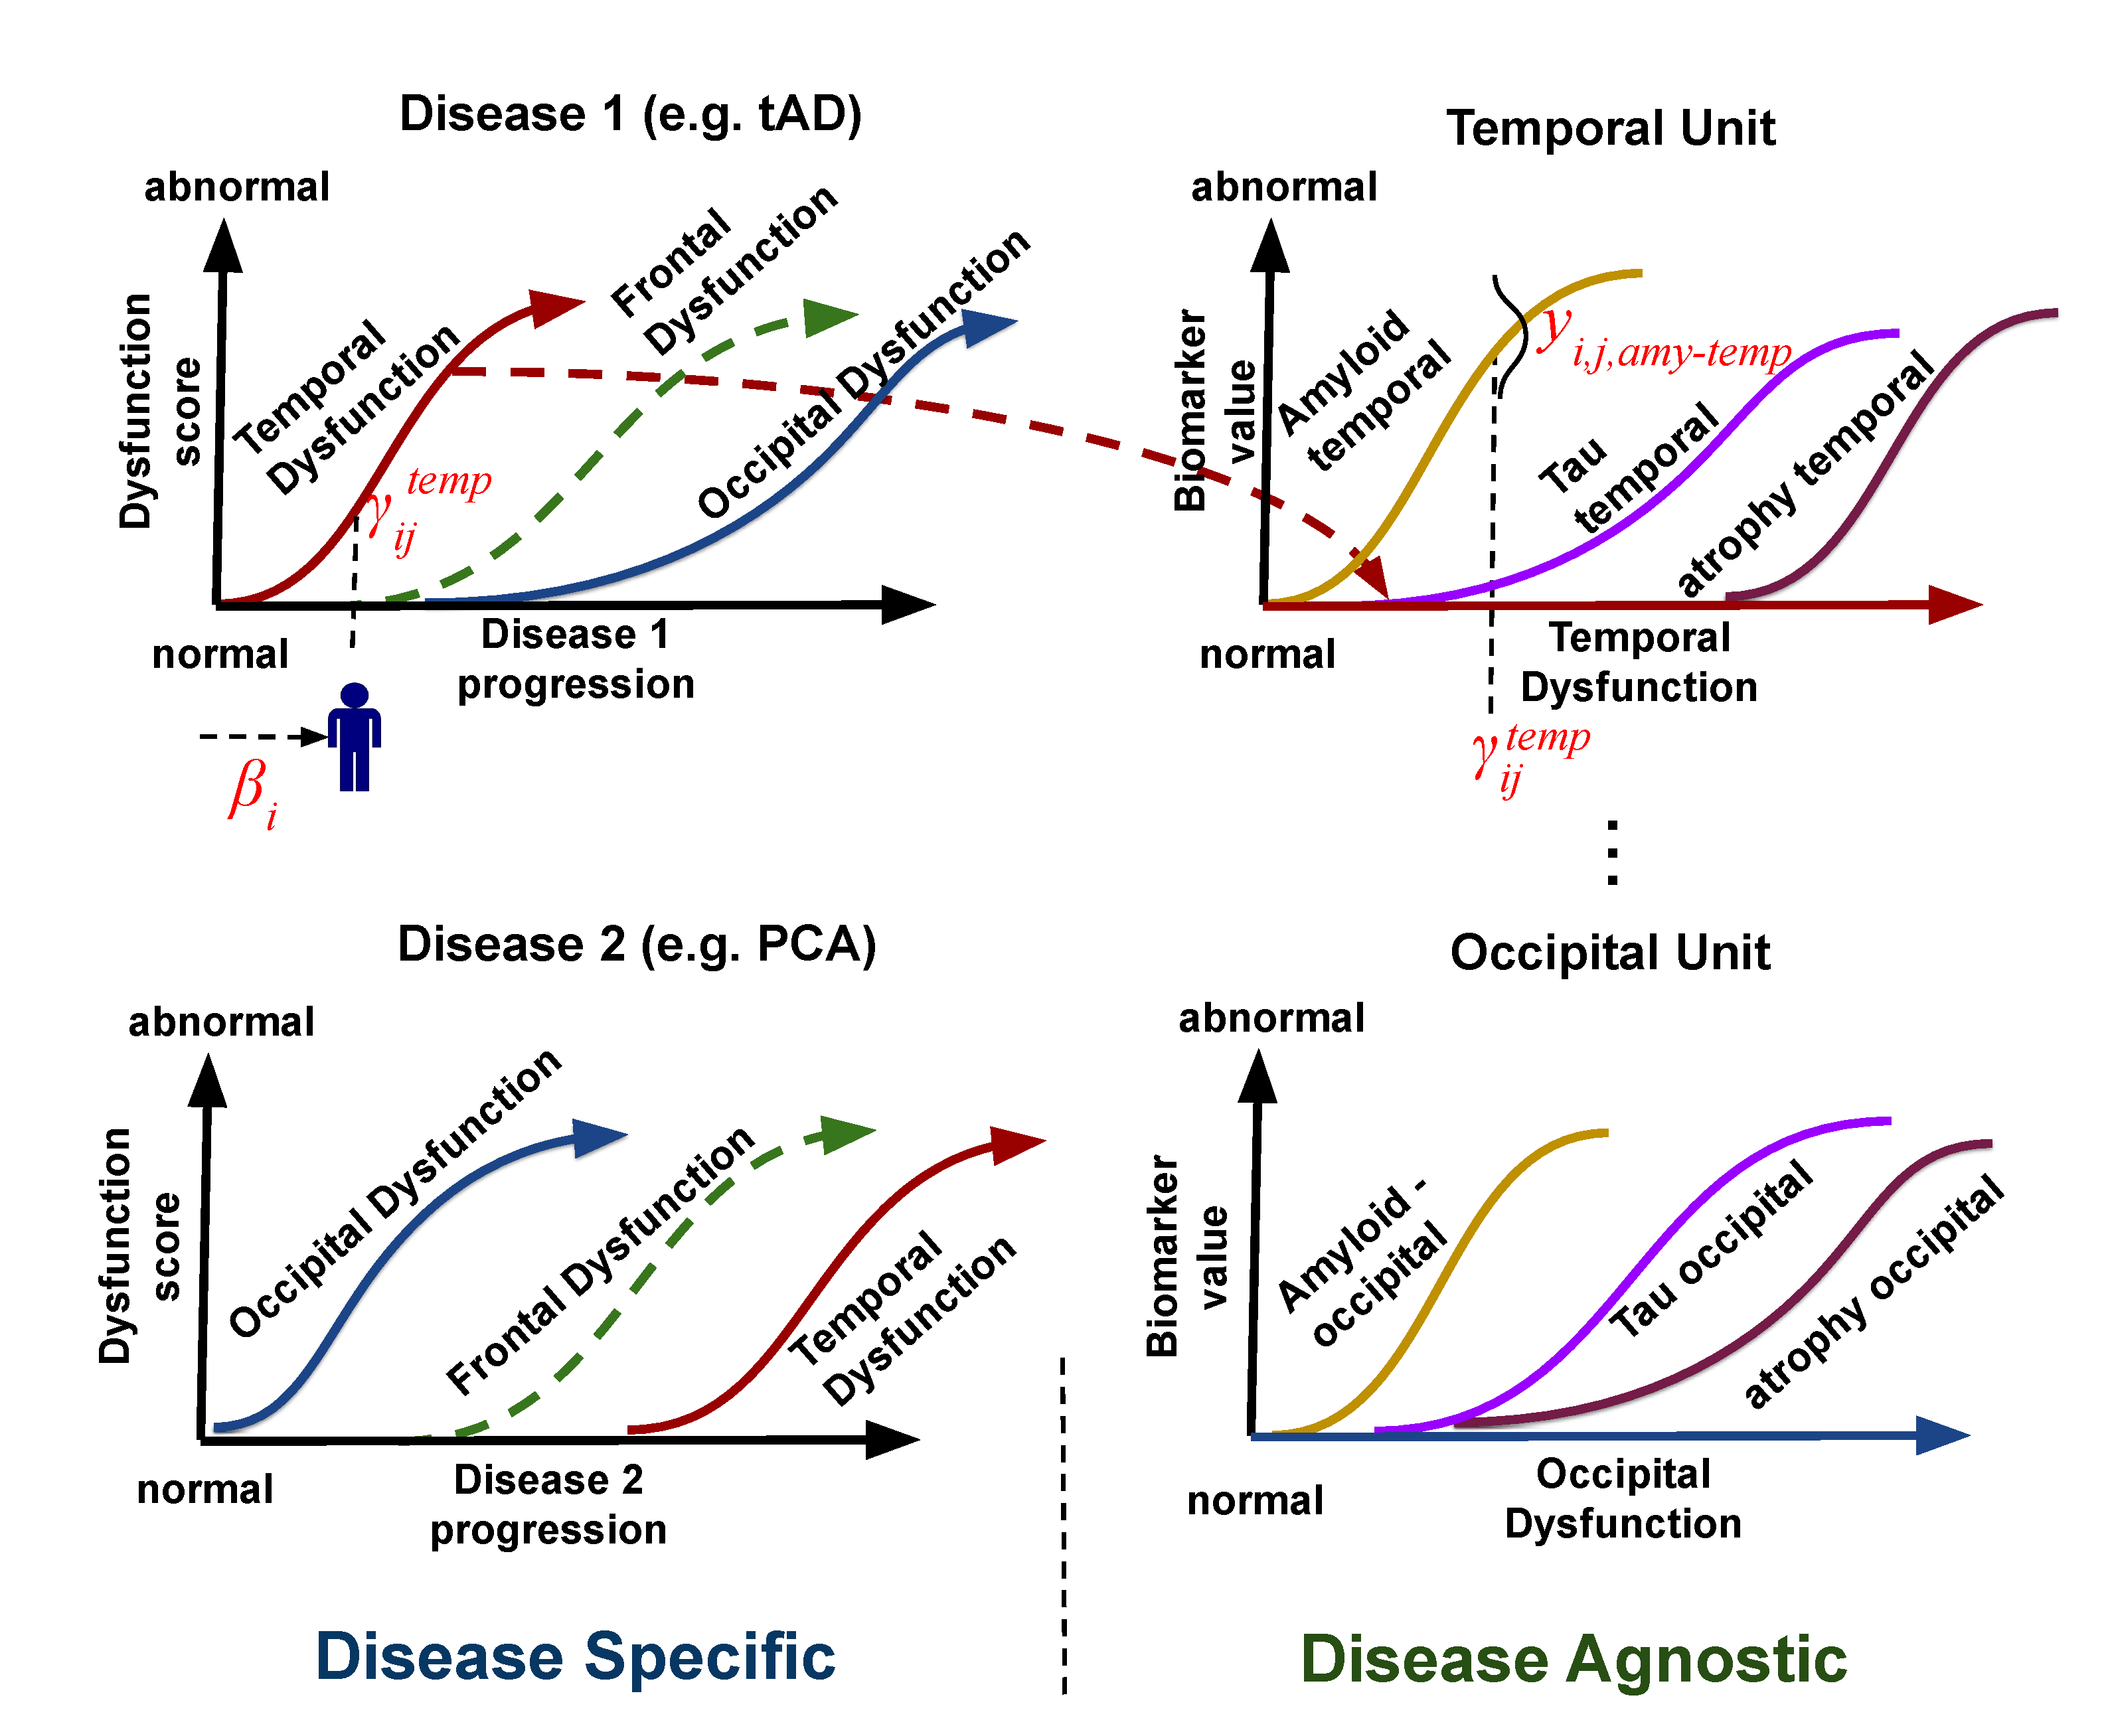
\includegraphics[width=\columnwidth]{disease_knowledge_transfer_poster.pdf}
  \fnt{3. Extend to multiple subjects, biomarkers and diseases}\\
 $ p(\boldsymbol{y}|\theta, \lambda, \beta , \epsilon) = \prod_{(i,j,k) \in \Omega} p(y_{ijk}|\theta_k, \lp, \beta_{i}) $
 \end{figure}


\columnbreak


\heading{3. Inference with belief propagation} 

% TODO bold out the diferences

\newcommand{\uu}{^{(u)}}
\newcommand{\um}{^{(u-1)}}

\newcommand{\algoFnt}[1]{\Large{#1}}

% \begin{itemize}
%  \item Uses loopy belief propagation
% \end{itemize}

\begin{figure}[H]
\begin{algorithm}[H]
\algoFnt{
%  Initialise $\boldsymbol{\theta}^{(0)}$, $\boldsymbol{\lambda}^{(0)}$, $\boldsymbol{\beta}^{(0)}$\\
  \While{$\boldsymbol{\theta}$, $\boldsymbol{\lambda}$, $\boldsymbol{\beta}$ not converged}{
   \tcp*[l]{\algoFnt{Estimate biomarker trajectories (disease agnostic)}}
%     \For{$k=1$ to $K$}{
      ${\theta_k\uu = \argmin_{\theta_k} \textcolor{red}{\sum_{(i,j) \in \Omega_k}} \left[y_{ijk} - g\left(f(\beta_i\um + m_{ij}; \lpum) ; \theta_k\right) \right]^2 }$\\
%       ${\epsilon_k\uu = \frac{1}{|\Omega_k|} \sum_{(i,j) \in \Omega_k}    \left[y_{ijk} - g\left(f(\beta_i\um + m_{ij}; \lpum) ; \theta_k\uu \right) \right]^2 }$\\
%     }
     \tcp*[l]{\algoFnt{Estimate dysfunction trajectories (disease specific)}} 
%     \For{$d=1 \in \mathbb{D}$}{
%       \For{$l=1 \in \Lambda$}{
        ${\lambda_{d}^{l, (u)} = \argmin_{\lambda_{d}^{l}} \textcolor{red}{\sum_{(i,j,k) \in \Omega_{d,l}}} \left[y_{ijk} - g\left(f(\beta_i\um + m_{ij}; \lambda_{d}^{l}) ; \theta_k\uu 
        \right) \right]^2 }$\\
%       }
%     }
    \tcp*[l]{\algoFnt{Estimate subject-specific time shifts}} 
%     \For{$i=1 \in [1, \dots, S]$}{
      ${\beta_i\uu = \argmin_{\beta_i} \textcolor{red}{\sum_{(j,k) \in \Omega_i}} \left[y_{ijk} - g\left(f(\beta_i + m_{ij}; \lpuu) ; \theta_k\uu
      \right) \right]^2 }$\\
%     }
}
}
% \normalfont
\end{algorithm}
% \caption[The algorithm for estimating the DKT parameters]{The algorithm used to estimate the DKT parameters, based on loopy belief-propagation.}
\label{fig:dktAlgo}
\end{figure}



\heading{4. Datasets}

\begin{itemize}
 \item Dementia Research Center cohort: MRI scans from 76 PCA, 67 tAD, 87 controls for training, 10 PCA with DTI for validation.
 \item TADPOLE dataset (ADNI) split into three subgroups with different progressions: 21 hippocampal, 35 cortical, 27 subcortical.
%  \item Synthetic dataset mimicking the cohorts above: 50 subjects with "synthetic PCA", 100 subjects with "synthetic AD".
\end{itemize}


\vspace{0.6em}
\heading{5. Results}

% \vspace{0.6em}
\begin{itemize}
%  \item \fnt{In synthetic experiment, the estimated parameters are close to the true parameters.}
% \begin{figure}[H]
% 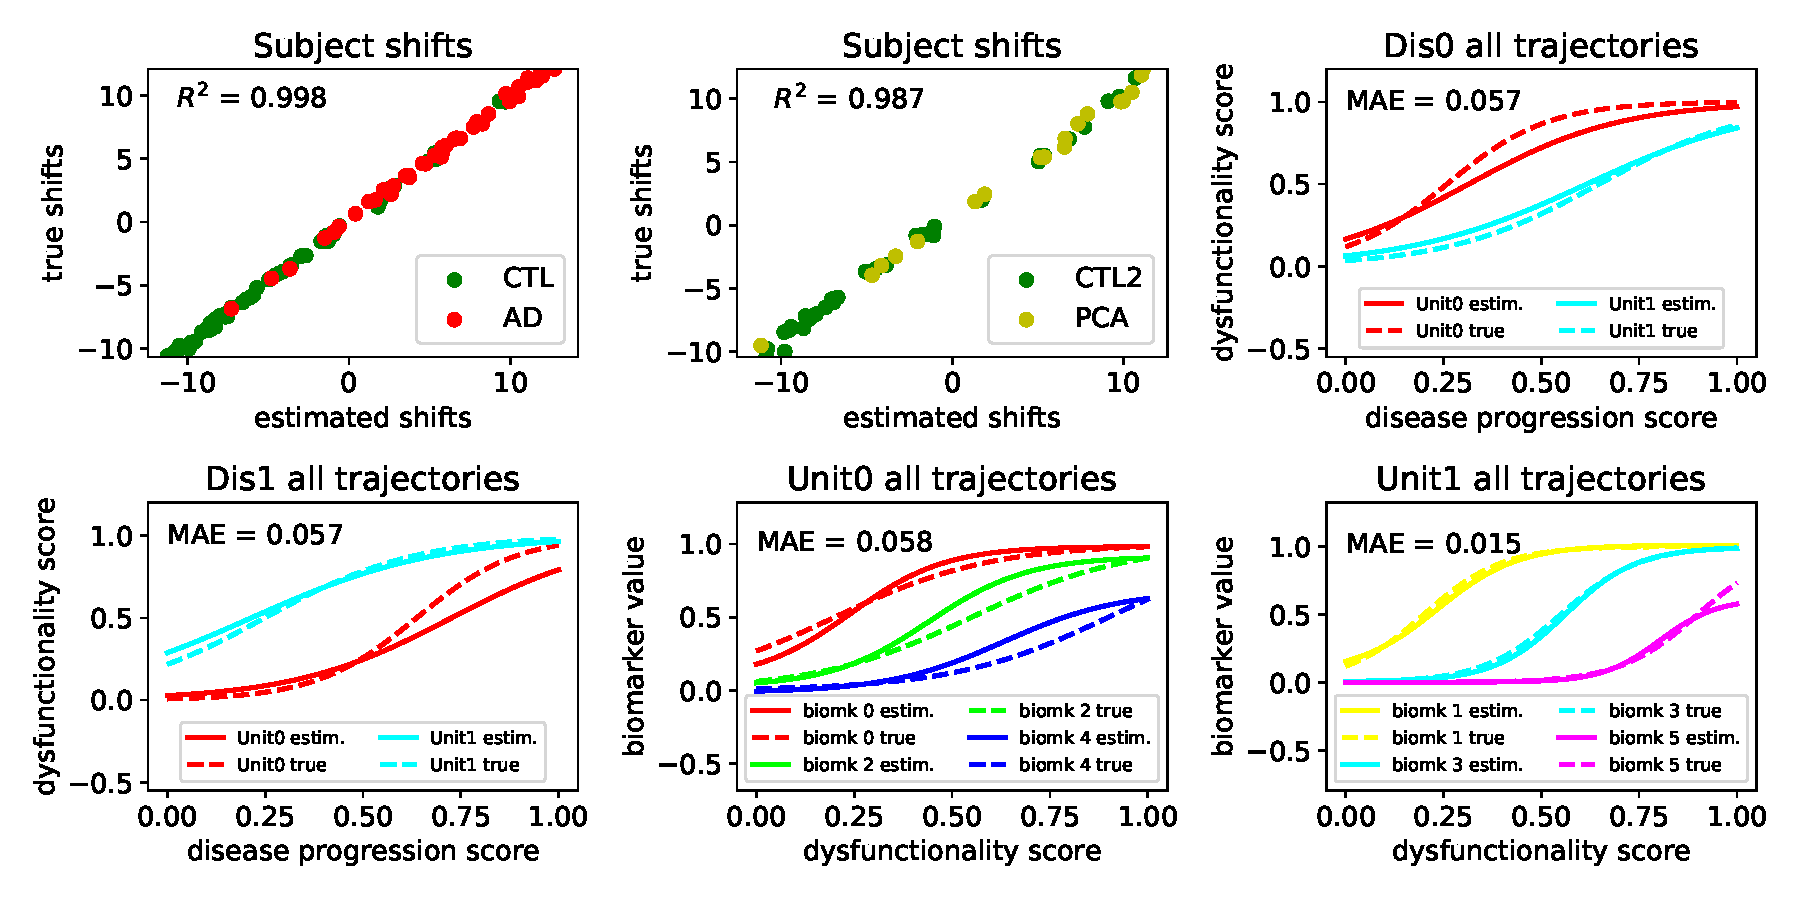
\includegraphics[width=\columnwidth]{../figures/compTrueParams105_synth1_JMD.pdf}
%   \label{fig:dktSynthTrajCompTrue}
% \end{figure}

 \item \fnt{Inferred multimodal trajectories for PCA in lack of such data.}
 \item \fnt{Results are plausible, suggesting late-stage posterior damage. }
\begin{figure}[H]
% \centering

 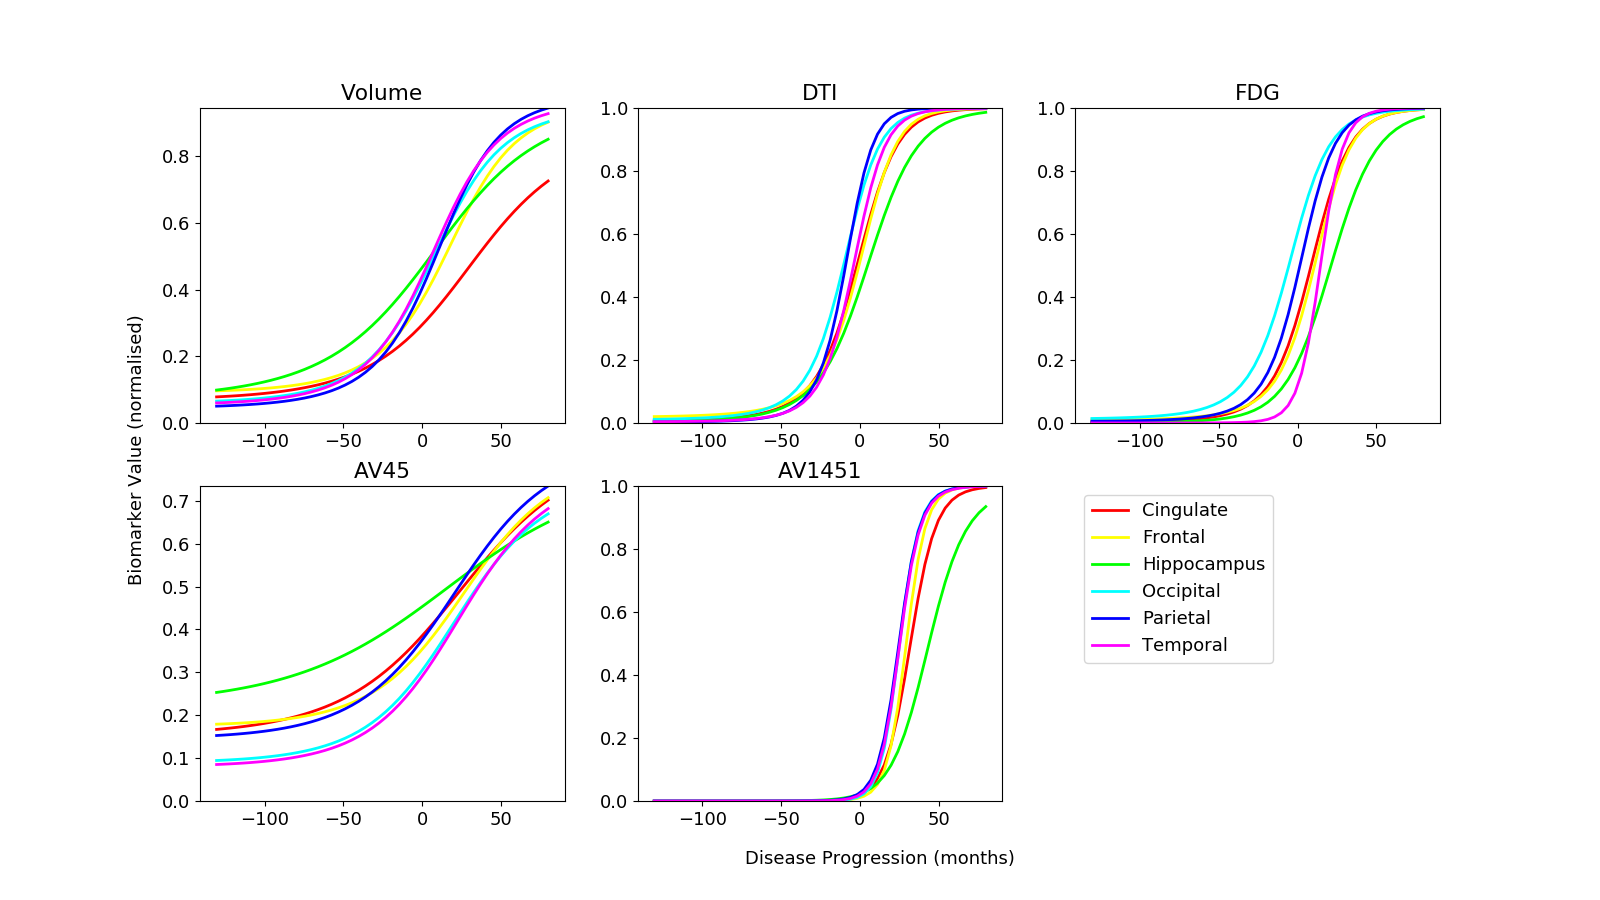
\includegraphics[width=\columnwidth, trim=0 20 0 35, clip]{../figures/trajDisSpaceOverlap_PCA_tad-drcTinyPen5_JMD.png}
%  \caption{Estimated trajectories for the PCA cohort. The only data that were available were the MRI volumetric data. The dynamics of the other biomarkers has been inferred by the model using data from typical AD, and taking into account the different spatial distribution of pathology in PCA vs tAD. }
%  \label{fig:PCAtrajByModality}
\end{figure}


\item \fnt{Our model has favourable performance compared to other models, on two different datasets.}
\vspace{0.3em}
\begin{figure}[H]
\fontsize{27}{30}\selectfont
\begin{tabular}{c | c c c c c c}
\textbf{Model} & \textbf{Cingulate} & \textbf{Frontal} & \textbf{Hippocam.} & \textbf{Occipital} & \textbf{Parietal} & \textbf{Temporal}\\
& \multicolumn{6}{c}{\textbf{TADPOLE: Hippocampal subgroup to Cortical subgroup}}\\
DKT (ours) &      0.56 $\pm$ 0.23 &    \textbf{0.35 $\pm$ 0.17} &        \textbf{0.58 $\pm$ 0.14} &     -0.10 $\pm$ 0.29 &     \textbf{0.71 $\pm$ 0.11} &     \textbf{0.34 $\pm$ 0.26} \\
AD model &      0.44 $\pm$ 0.25 &    0.34 $\pm$ 0.21 &       0.34 $\pm$ 0.24* &     \textbf{-0.07 $\pm$ 0.22} &     0.64 $\pm$ 0.16 &    0.08 $\pm$ 0.24* \\
Multivariate &      \textbf{0.60 $\pm$ 0.18} &   0.11 $\pm$ 0.22* &       0.12 $\pm$ 0.29* &     -0.22 $\pm$ 0.22 &   -0.44 $\pm$ 0.14* &   -0.32 $\pm$ 0.29* \\
Spline &    -0.24 $\pm$ 0.25* &  -0.06 $\pm$ 0.27* &        0.58 $\pm$ 0.17 &     -0.16 $\pm$ 0.27 &    0.23 $\pm$ 0.25* &    0.10 $\pm$ 0.25* \\
Linear &    -0.24 $\pm$ 0.25* &   0.20 $\pm$ 0.25* &        0.58 $\pm$ 0.17 &     -0.16 $\pm$ 0.27 &    0.23 $\pm$ 0.25* &    0.13 $\pm$ 0.23* \\
& \multicolumn{6}{c}{\textbf{typical Alzheimer's to Posterior Cortical Atrophy}}\\
DKT (ours) &    0.77 $\pm$ 0.11 &    0.39 $\pm$ 0.26 &      0.75 $\pm$ 0.09 &    0.60 $\pm$ 0.14 &    \textbf{0.55 $\pm$ 0.24} &    \textbf{0.35 $\pm$ 0.22} \\
AD model &    \textbf{0.80 $\pm$ 0.09} &    \textbf{0.53 $\pm$ 0.17} &      \textbf{0.80 $\pm$ 0.12} &    0.56 $\pm$ 0.18 &    0.50 $\pm$ 0.21 &    0.32 $\pm$ 0.24 \\
Multivariate &   0.73 $\pm$ 0.09 &   0.45 $\pm$ 0.22  &    0.71 $\pm$ 0.08 & -0.28 $\pm$ 0.21* &  0.53 $\pm$ 0.22  &  0.25 $\pm$ 0.23* \\
Spline &   0.52 $\pm$ 0.20* &  -0.03 $\pm$ 0.35* &     0.66 $\pm$ 0.11* &   0.09 $\pm$ 0.25* &    0.53 $\pm$ 0.20 &   0.30 $\pm$ 0.21* \\
Linear &   0.52 $\pm$ 0.20* &    0.34 $\pm$ 0.27 &     0.66 $\pm$ 0.11* &    \textbf{0.64 $\pm$ 0.17} &    0.54 $\pm$ 0.22 &   0.30 $\pm$ 0.21* \\
\end{tabular}
\vspace{0.5em}
% \caption[Performance evaluation of DKT and other models]{Performance evaluation of DKT and four other statistical models of decreasing complexity. }
% \end{footnotesize}
\label{sec:dktPerfMetrics}
\end{figure}


\end{itemize}

\heading{6. Conclusion}

\begin{itemize}
 \item Developed a novel methodology and model for transfer learning across different diseases
 \item Inferred multimodal trajectories for Posterior Cortical Atrophy
%  \item 
\end{itemize}





\end{multicols}
\hrule


}


\begin{multicols}{2}

\Large{

\raggedcolumns	


\vspace{-1em}
\subsection*{Weblinks}
\begin{itemize}
\item Source code: \url{https://github.com/mrazvan22/dkt}
\item Website: \url{https://people.csail.mit.edu/razvan/}
\end{itemize}
}



\columnbreak

\subsection*{Funders}

% \begin{figure}[H]
% \begin{subfigure}{0.48\columnwidth}
\vspace{0em}
% \hspace{2em}
\newcommand{\heightLogos}{3.5cm}

\includegraphics[height=\heightLogos]{epsrc_logo}
\hspace{0.5em}

\includegraphics[height=\heightLogos]{nac_logo} 
\hspace{0.5em}

\includegraphics[height=\heightLogos]{cdt_logo} 
\hspace{0.5em}

\includegraphics[height=\heightLogos]{nih_logo} 
\hspace{0.5em}

\includegraphics[height=\heightLogos]{aruk_logo} 
\hspace{0.5em}
% \end{subfigure}
% \begin{subfigure}{0.48\columnwidth}
%  \begin{itemize}
%  \item  EPSRC grant EP/L016478/1
%  \item  NIH grant NIBIB NAC P41EB015902
% \end{itemize}
% \end{subfigure}

% \end{figure}



\end{multicols}


\end{document}
